\documentclass[a4paper,11pt,fleqn]{article}%fleqn pour aligner les equations à gauche
\usepackage{../../Styles/Exercice}


\newcommand{\chnum}{Chapitre 16}
\newcommand{\chtitle}{Thermodynamique}
\newcommand{\dtype}{Exercices}
  

\begin{document}
	\maketitle
\begin{multicols}{2}
\section{Déterminer une variation d'énergie interne}
De l'eau dans une baignoire de volume $V = \SI{200}{L}$ est chauffée de \SI{15}{\celsius} à \SI{37}{\celsius}.\\
\textbf{Données :}
\begin{itemize}
	\item Masse volumique de l'eau : $\rho_{eau} = \SI{1,00E3}{\kilo\gram\per\meter\cubed}$
	\item Capacité thermique massique de l'eau : $c_{eau} = \SI{4180}{\joule\per\kelvin\per\kilo\gram}$
\end{itemize}
\begin{enumerate}
	\item Comparer qualitativement l'énergie cinétique des molécules d'eau à l'état initial et à l'état final.
	\item Préciser comment évolue l'énergie interne du système \{eau\} lors du chauffage de l'eau.
	\item Déterminer l'énergie nécessaire pour chauffer l'eau.
	\item Calculer la durée de fonctionnement d'une ampoule de \SI{10}{W} avec cette énergie. Commenter.
\end{enumerate}

\section{Bilan énergétique dans un sauna}
Un homme se trouve dans la cabine d'un sauna. Un radiateur électrique est utilisé pour compenser les pertes thermiques $Q_e$ avec l'extérieur (air extérieur, homme, etc. ) et maintenir ainsi constante la température de la cabine.\\
\textbf{Données :}\\
Transferts d'énergie pendant la durée d'utilisation du sauna :
\begin{itemize}
	\item Travail électrique reçu par le radiateur $\mathcal{W}_r = \SI{12E6}{J}$
	\item Transfert thermique entre la cabine et l'extérieur $|Q_e| = \SI{13E6}{J}$
\end{itemize}
\begin{enumerate}
	\item Représenter sur un schéma les transferts d'énergie liés au système \{cabine\} et déterminer le signe des valeurs de ces transferts.
	\item Appliquer le premier principe de la thermodynamique au système \{cabine\} et déterminer l'expression de la variation de l'énergie interne $\Delta \mathcal{U}$ du système en fonction de $Q_e$ et $\mathcal{W}_r$.
	\item Calculer la valeur de la variation d'énergie interne $\Delta \mathcal{U}$ du système \{cabine\}. Préciser si le radiateur permet de compenser entièrement les pertes thermiques. Justifier.
\end{enumerate}

\section{Fonctionnement d'une bouilloire}
Un échantillon d'eau de masse $m=\SI{700}{g}$, de température $\theta_i=\SI{20}{\celsius}$, est porté à ébullition dans une bouilloire en une durée $\Delta t =\SI{3}{min}$.\\
Le schéma des transferts est donné ci-contre, pour le système \{eau\}.\\
\textbf{Données :}\\
\begin{itemize}
	\item Capacité thermique massique : $c_{eau} =\SI{4,18}{\kilo\joule\per\kelvin\per\kilo\gram}$.
	\item Puissance électrique de la résistance de la résistance chauffante : $\mathcal{P} =\SI{1,5}{\kilo\watt}$.
\end{itemize}
\begin{enumerate}
	\item En supposant que l'intégralité de l'énergie électrique reçue par la résistance chauffante est utilisée pour chauffer l'eau, déterminer la valeur du transfert thermique $Q_1$.
	\item Calculer la variation de l'énergie interne de l'eau au cous de l'expérience.
	\item En déduire la valeur du transfert thermique $Q_2$ vers l'extérieur. Commenter son signe.
\end{enumerate}

\section{Combinaison de plongée}
L'un des problèmes rencontrés par un plongeur est le choix d'une combinaison adaptée à la température de l'eau et à la durée de la plongée. Il doit en effet éviter l'hypothermie : si la température interne baisse de \SI{1}{\celsius}, il doit immédiatement remonter à la surface.\\
Un plongeur de masse $m=\SI{80}{\kilo\gram}$ est entièrement immergé dans l'eau de température uniforme et constante $\theta_{eau} = \SI{4}{\celsius}$. La température interne initiale du plongeur est $\theta_0=\SI{37}{\celsius}$. Sa température interne au cours du temps est notée $\theta (t)$.\\
Le plongeur est naturellement réchauffée par la thermogenèse (puissance générée par des transformations métaboliques). La puissance associées à cette thermogenèse est ici supposée constante et vaut $\mathcal{P}_{th}=\SI{200}{W}$.\\
Les échanges thermiques entre l'eau et le plongeur sont de type conducto-convectifs et peuvent être modélisés par la loi phénoménologique de Newton : $$\phi_{cc}(t) = h \cdot S \cdot (\theta(t) - \theta_{eau})$$
Avec $S$ la surface de contact eau/plongeur et $h$ le coefficient d'échange conducto-convectif.\\
\textbf{Données :}
\begin{itemize}
	\item $S$ = \SI{1}{\meter\squared}
	\item Sans combinaison : $h_{nu} = \SI{100}{\watt\per\meter\squared\per\celsius}$
	\item Avec combinaison : $h_{combi} = \SI{8}{\watt\per\meter\squared\per\celsius}$
	\item Capacité thermique massique du corps humain : $c =\SI{3,5E3}{\joule\per\kilo\gram\per\celsius}$
\end{itemize}
\begin{enumerate}
	\item Réaliser un bilan d'énergie sur le système \{plongeur sans combinaison\} et donner l'expression de sa variation d'énergie interne $d\mathcal{U}$ pendant une durée élémentaire $dt$ en fonction de $\mathcal{P}_{th}$ et de $\Phi_{cc}$.
	\item En déduire que la température interne $\theta(t)$ du plongeur vérifie l'équation différentielle suivante :
	$$\dfrac{d\theta}{dt} + \dfrac{1}{\tau}\theta = \dfrac{\theta_{eau}}{\tau} + \dfrac{\mathcal{P}_{th}}{mc} $$
	où $\tau$  est une constante dont l'expression est à déterminer.
	\item Résoudre cette équation différentielle et donner l'expression de $\theta(t)$.
	\item Déterminer la durée maximale de plongée envisageable avec et sans combinaison. Commenter les résultats. 
\end{enumerate}
%\newpage
\section{Étude énergétique d'une centrale nucléaire}
Une centrale nucléaire est le lieu de nombreux transferts d'énergie dans lesquels l'eau joue un rôle important.\\
\begin{centering}
	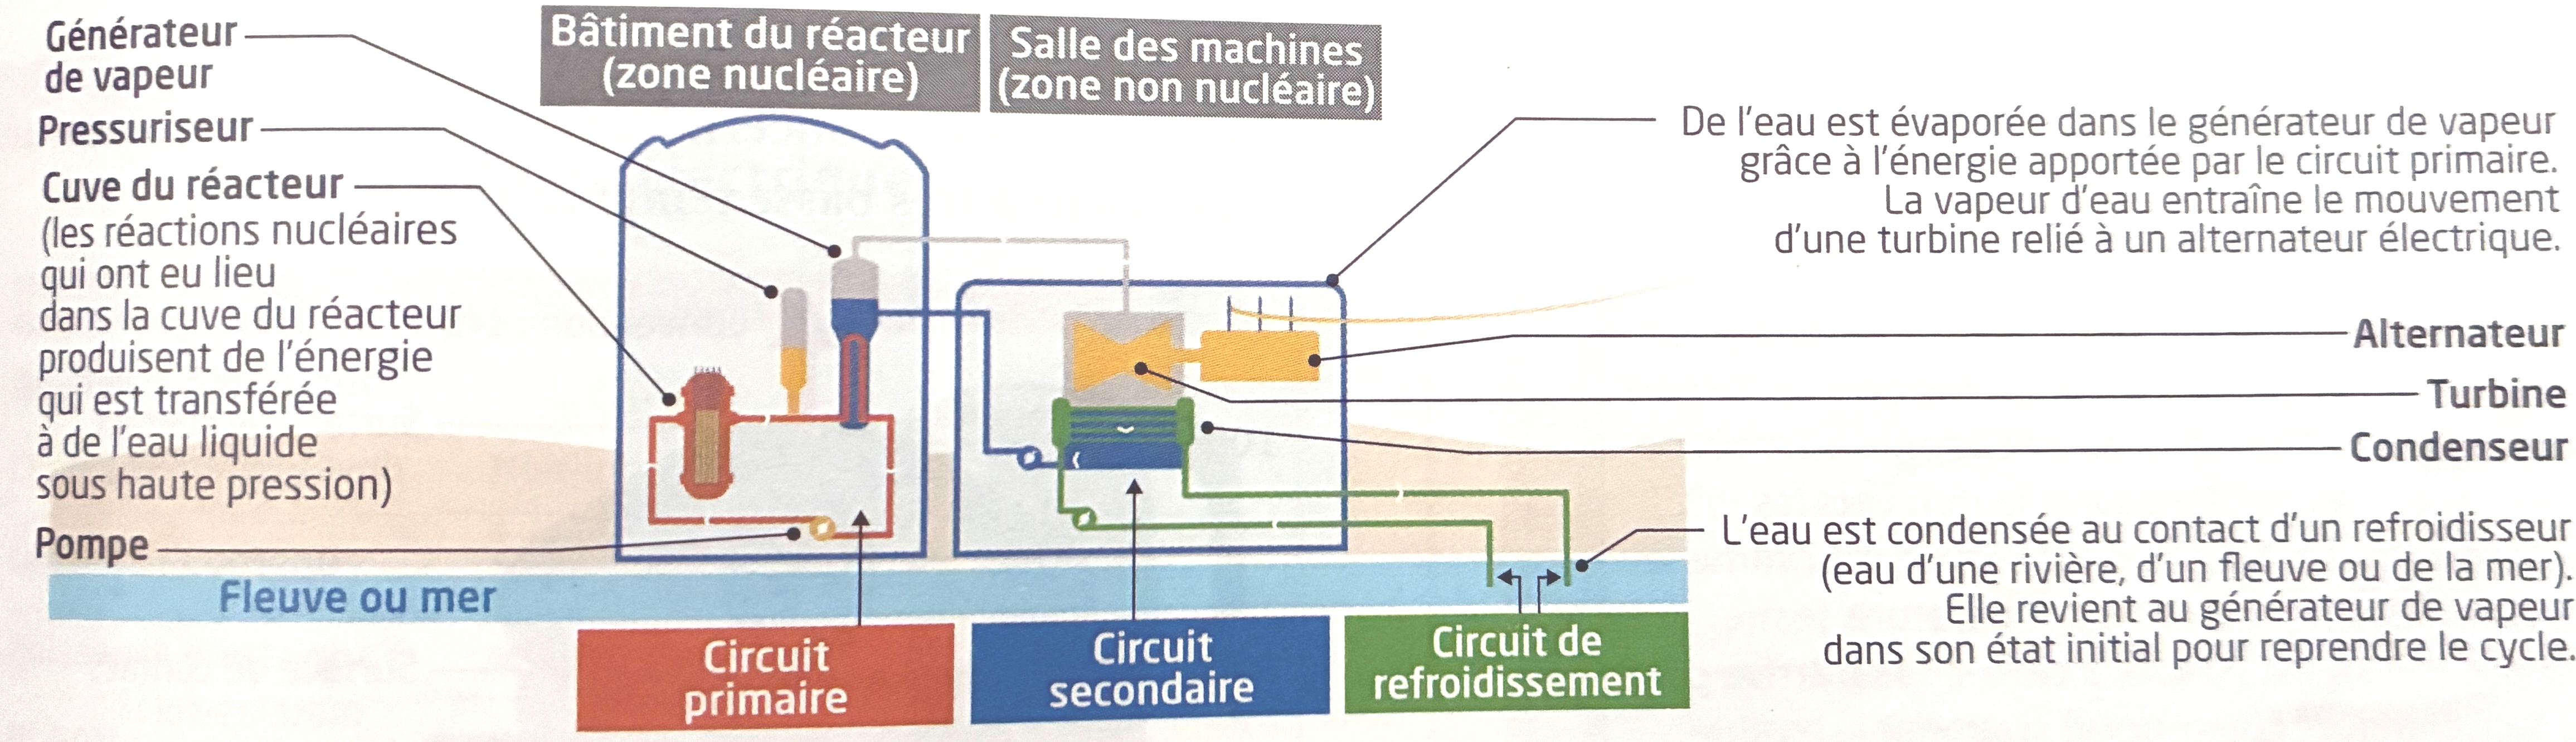
\includegraphics[width=\linewidth]{Ressources/TSPE_C14_Exercices_Fig2.png}
\end{centering}
\noindent \begin{minipage}{\linewidth}
	\textbf{Données :}
	%\begin{multicols}{2}
		\begin{itemize}
			\item Capacité thermique massique de l'eau $c_{pm}$ dans différentes conditions :
		\end{itemize}
		\begin{tabular}{|>{\centering}m{.3\linewidth}|>{\centering}m{.2\linewidth}|>{\centering}m{.13\linewidth}|>{\centering\arraybackslash}m{.2\linewidth}|}
		\hline
		\textbf{Température (en \unit{\celsius})} & \textbf{Pression (en bar)} & \textbf{État} & \textbf{$\mathbf{c_{pm}}$ (en \unit{\joule\per\kelvin\per\kilo\gram})}\\
		\hline \num{270} & \num{155} & Liquide & \num{5250}\\
		\hline \num{10} & \num{1} & Liquide & \num{4180}\\
		\hline \num{270} & \num{56} & Gaz & \num{3800}\\
		\hline		
		\end{tabular}
		\begin{itemize}
			\item Puissance électrique fournie par la centrale nucléaire : $\mathcal{P}_e = \SI{900}{\mega\watt}$.
			\item Rendement de la centrale nucléaire : $\eta = \SI{33}{\percent}$
			\item Diagramme présentant les états de l'eau en fonction de la température et de la pression :
		\end{itemize}
		\begin{center}
			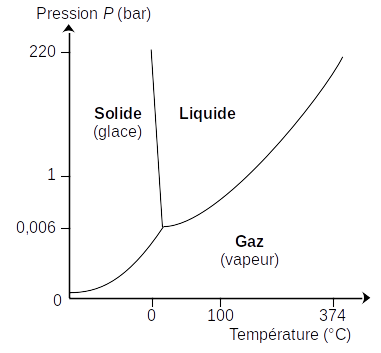
\includegraphics[width = .9\linewidth]{Ressources/TSPE_C14_Exercices_Fig1.png}
		\end{center}
	%\end{multicols}
\end{minipage}\\

\begin{enumerate}
	\item \textbf{Transferts d'énergie dans le circuit primaire}
	\begin{enumerate}
		\item Calculer l'énergie fournie chaque seconde par le réacteur nucléaire et préciser le mode de transfert thermique par lequel cette énergie est échangée avec l'eau du circuit primaire.
		\item En analysant les données, justifier le choix d'utiliser de l'eau liquide dans le circuit primaire, ainsi que de travailler à haute pression.		
	\end{enumerate}
	\item \textbf{Transferts d'énergie dans le circuit secondaire}\\
	L'énergie fournie par le réacteur nucléaire est supposée intégralement transférée au circuit primaire, puis au circuit secondaire.
	\begin{enumerate}
		\item  Schématiser les différents transferts d'énergie liés au système \{eau du circuit secondaire\}. Préciser le signe de chacun des transferts représentés sur ce schéma.
		\item Comment varie l'énergie interne $\mathcal{U}$ du système \{eau du circuit secondaire\} au cours du cycle ?
		\item Montrer que le flux thermique entre le circuit secondaire et le circuit de refroidissement vaut \SI{1,8}{\giga\watt}.
	\end{enumerate}
	\item \textbf{Transferts d'énergie dans le circuit de refroidissement}\\
	L'eau du fleuve est récupérée par pompage, puis envoyée dans la canalisation avec un débit volumique constant $D_V = \SI{60}{\meter\cubed\per\second}$. La température de l'eau du fleuve à l'entrée du circuit de refroidissement est $\theta_e=\SI{19}{\celsius}$. Déterminer la température $\theta_s$ de l'eau à la sortie de la canalisation. 
\end{enumerate}

\section{Piscine municipale}
On souhaite remplir le bassin d'une piscine de \SI{500}{\meter\cubed} d'eau à une température de $\theta_p = \SI{28}{\celsius}$. On ne dispose que d'une arrivée d'eau froide à $\theta-f = \SI{20}{\celsius}$ et d'une arrivée d'eau chaude à $\theta_c=\SI{60}{\celsius}$. On simplifie le calcul en considérant que l'eau, une fois dans le bassin, se comporte comme un système isolé.
\begin{enumerate}
	\item Déterminer la relation entre la variation d'énergie interne de l'eau froide $\Delta U_t$ et la variation d'énergie interne de l'eau chaude $\Delta U_c$ entre leur état initial et l'état final.
	\item En déduire les masses d'eau à mélanger.
\end{enumerate}
\textbf{Données :}
\begin{itemize}
	\item \textbf{Capacité thermique massique de l'eau :} $c = \SI{4,79}{\kilo\joule\per\kilo\gram\per\kelvin}$
	\item \textbf{Masse volumique de l'eau :} $\rho = \SI{998}{\kilo\gram\per\meter\cubed}$
\end{itemize}

\section{\OE uf parfait}
Très prisé par les fins gourmets, l'\oe uf parfait est un \oe uf cuit exactement à sa température de coagulation $\theta = \SI{64,5}{\celsius}$, pendant \SI{45}{\minute}, à la casserole.
\begin{enumerate}
	\item Donnner un ordre de grandeur de l'énergie reçue nécessaire à l'élévation de la température du système jusqu'à la température de coagulation.
	\item Une fois la température atteinte, on suppose que le système cède à l'extérieur une puissence égale à \SI{80}{\watt}. Déterminer l'énergie $Q$ nécessaire au maintien de cette température pendant \SI{45}{\minute}.\\
	\textbf{Données :}
	\begin{itemize}
		\item \textbf{Masse volumique de l'eau :} $\rho_{eau} = \SI{1,0E3}{\kilo\gram\per\meter\cubed}$
		\item \textbf{Capacité thermique massique de l'\oe uf :} $c=\SI{3,3}{\kilo\joule\per\kilo\gram\per\kelvin}$
		\item \textbf{Capacité thermique massique de l'eau :} $c_{eau} = \SI{4,2}{\kilo\joule\per\kilo\gram\per\kelvin}$
		\item \textbf{Masse de l'\oe uf :} $m = \SI{57}{\gram}$
		\item \textbf{Volume d'eau dans la casserole :} $V_{eau} = \SI{1,5}{\liter}$
	\end{itemize}
\end{enumerate}

\section{Équilibre d'une montgolfière}
Une montgolfière est immobile dans l'atmosphère.
\begin{itemize}
	\item Déterminer la température de l'air à l'intérieur de l'enveloppe. On considère que l'air se comporte comme un gaz parfait.
\end{itemize}
\textbf{Données :}
\begin{itemize}
	\item \textbf{Masse de l'ensemble (nacelle + brûleur + enveloppe + passagers) :} $m_{tot} = \SI{500}{\kilo\gram}$
	\item \textbf{Volume de l'envelopper :} $V=\SI{2000}{\meter\cubed}$
	\item \textbf{Conditions atmosphérique :} $\rho_O = \SI{1,013}{\bar}$ et $\theta_O = \SI{12,0}{\celsius}$
	\item \textbf{Masse molaire de l'air :} $M = \SI{29,0}{\gram\per\mole}$
	\item \textbf{Constante des gaz parfaits :} $R = \SI{8,314}{\joule\per\kelvin\per\mole}$
\end{itemize}
\end{multicols}
\end{document}